%! TEX root = 'main.tex'

%\section{Experiments}

\section{Implementation}
\label{sec:implementation}

In this section, we give some implementation details and issues that we had during development.

\subsection{Hypervisor}


There are two new modes to run under virtualization: VMX root operation and VMX non-root operation. VMX stands for virtual machine extension. It proves new instructions VMXON, VMXOFF, VMPTRLD, VMPTRST, VMCLEAR, VMREAD, VMWRITE, VMCALL, VMLAUNCH, VMRESUME.

Usually processor has running mode known as ring-0 to ring-3, where ring-0 is kernel mode, ring-3 is user mode, ring 1 and ring 2 are rarely used. When CPU enables virtualization, it could be seen as running in the non-root mode. The root mode can be considered as a lower and more privileged level, it controls the whole CPU. And the guest operating system will run in non-root mode. Root mode runs VMM (Virtual Machine Monitor) is often called ring -1.

VMXON and VMXOFF are instructions to enter and exit VMX mode. There is an important data structure called VMCS (Virtual-Machine Control Structure), which is 4 KB large in size. It controls the state switch between VMX root mode and VMX non-root mode. From root mode to non-root mode called VM Exit. From non-root mode to root mode called VM Enter.

Every logical CPU (each core in a real physical CPU is called a logical CPU) has a processor state called VMCS pointer. It contains the physical address of the VMCS. There could be many VMCSs, the one stored in VMCS pointer is considered as the current one. Every VMCS can represent a virtual processor for the virtual machine, inside virtual machine, that is a logical CPU seen by operating system. Although hypervisor knows the physical address of a VMCS, but hypervisor cannot modify it directly, hypervisor can only reads and writes VMCS using VMREAD, VMWRITE instructions. Hypervisor use VMPTRLD to set a VMCS both as active and current. And use VMCLEAR to mark the VMCS as inactive.

A VMCS contains many fields related every aspect of a virtual machine. There are six fields: Guest-state area, Host-state area, VM-execution control fields, VM-exit control fields, VM-entry control fields and VM-exit information fields. And each field also contains many more control fields with a lot of settings. Once the CPU enters into a virtual machine by execute VMLAUNCH which associates with a VMCS, this virtual machine is fully control by the settings in the VMCS. For example, the CR4 field in the Guest-state area is the one we used to update the actual CPU register.  Hypervisor can set during what circumstances the virtual machine should exit. And then the hypervisor can handle this situation, for example emulate a hardware device or change the virtual machine's behavior. In this case, it's the control register related operations that we are interested. 

We do not actually emulate any hardware device, we put the current system into a virtual machine environment and our code run as the hypervisor.

\subsection{Page Faults}
Handling exceptions is the major part of this mitigation. The type we need to handle is page fault exception. They may be caused directly by SMAP or by our protection on the pages. Even though it's called "page fault", but not all exceptions are due to program errors. For example, page fault is one part of paging mechanism in x86 architecture to make the virtual memory much larger then the physical memory that exists in the system. 

We need to handle all the page fault exceptions before the system's handler does. Some of the them need to be passed to the operating system, for example, those invalid pages. And the others need to be intercepted. There is a 32-bit error code being pushed into the kernel stack when exception triggered, as shown in~\autoref{fig:pagefaulterrorcode}.


\begin{figure}[th]
  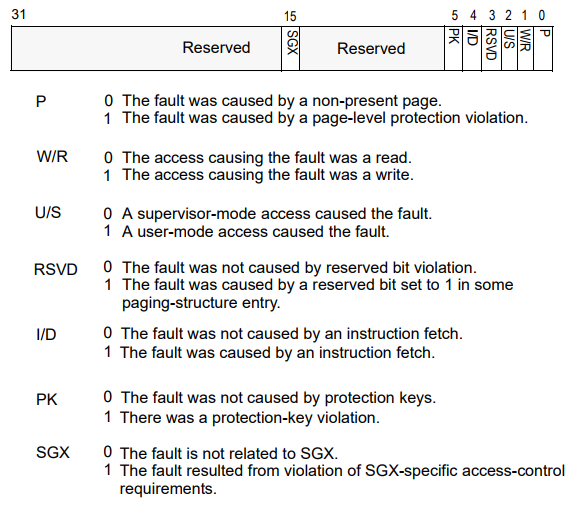
\includegraphics[width=0.47\textwidth]{figures/pagefaulterrorcode}
  \centering
  \caption{Page Fault Error Code.~\cite{intelinterrupt} Unfortunately, SMAP doesn't have a separate bit. The exception it triggers comes with U/S bit set to 0, but the reason for that is not unique.}
  \label{fig:pagefaulterrorcode}
\end{figure}

The bits don't clearly indicate the cause. For example, there is no "SMAP" bit. So our page fault handler needs to collect more information in order to tell the possible reason for the exception. Register values of EIP, CS, ESP, SS, EFLAGS are also pushed into the kernel stack with the error code. We also get the page table root from CR3 and the faulting virtual address from CR2.

First, We need to screen out some of the cases that are irrelevant. For example, When exceptions come in with "P" bit unset, indicating that the page is not present in the memory. It's part of the paging mechanism, pages can be swapped out to secondary storage such as hard disk. Even our page fault handler itself may trigger this type of page faults. Since page tables are reside in the page-able pages, so when we walk through the page table, some of the PTE pages may not be there. Therefore we need to pass such page faults to operating system as soon as possible, otherwise it will cause a dead loop inside our handler. We also observe that there is no exception caused both by non-present page and SMAP at the same time, so it's safe to do so.

After screen out unrelated exceptions, the algorithm that handles mitigation related exceptions is shown in Algorithm~\ref{algo:pagefaulthandler}.


\begin{algorithm}[ht]
\begin{algorithmic}[1]
\small
\Procedure{PageFaultHandler}{}

\State $address\gets cr2$ 
\State $pte\gets \Call{\textbf{GET\_PTE}}{address}$
\State $teb\gets fs:0x18$

\If{$smap\_violation$}
	\State $pages[]\gets \Call{\textbf{ADD\_PAGE}}{$address, pte, cr3, teb$}$
    \State $\Call{\textbf{SET\_PAGE\_KERNEL}}{pte}$
    \State $\Call{\textbf{Flush\_TLB}}{address}$
    \State \Return{$re-execute$}
\ElsIf{$user\_access\_protected\_page$}
	\If{$error.WRITE$}
    	\Repeat 
        \State{$\Call{\textbf{SLEEP}}$}
        \If{$\Call{\textbf{Check\_Permits}}{pte}$}
        	\State \Return{$re-execute$}
        \EndIf
        \Until{$count < 10$}
        \State \Return{$terminate\_thread$}
    \Else
    	\State $\Call{\textbf{SET\_PAGE\_USER\_READONLY}}{pte}$
    	\State $\Call{\textbf{Flush\_TLB}}{address}$
        \State \Return{$re-execute$}
    \EndIf
%\ElsIf{$user\_write\_readonlypage$}
%	\If{\Call{HAS\_RECORD}{pte}}
%    \EndIf
\EndIf
\State \Return{$original\_handler$}
   
\EndProcedure
\end{algorithmic}
\normalsize
\caption{Page Fault Handler}
\label{algo:pagefaulthandler}
\end{algorithm}


Another technical detail we should mention is that when entering page fault handler, interrupts are tuned off automatically. This is because exception is raised through an "interrupt gate". The CPU clears the IF(Interrupt enable flag) in the EFLAGS register and sets it back when interrupts return. In our case, after getting the faulting virtual address from CR2, we immediately set the IF flag by executing instruction "STI" in order to let the processor being able to receive nested exceptions.

\subsection{Updating PTE}

To change page's attributes, we need to change the bits in the corresponding PTE. In a multi-processor system(SMP), updating global data needs to hold a global lock in order to synchronize with other threads. Since our module is a 3rd-party module to windows kernel, we don't have the information for the windows kernel's private variables such as the spinlock that synchronize the updating of page tables. 

In an attacking scenario, there will be at least two threads. One calls the victim kernel function, the other keeps modifying the user data that used by the victim kernel function. To win the race, normally the attacker needs to repeat the process as frequent as possible. So is our page fault handler. 

We need to make our operation atomic. As shown in~\autoref{fig:pte}, U/S bit controls whether the page is a user page of a kernel page. R/W controls whether the page is writable. The PTE data structure on 32-bit system is defined as the following:

%\begin{lstlisting}[style=code, float]
\begin{lstlisting}[style=code] 
typedef struct _PTE_HARDWARE
{
	ULONG Valid : 1;
	ULONG Write : 1;
	ULONG Owner : 1;
	ULONG WriteThrough : 1;
	ULONG CacheDisable : 1;
	ULONG Accessed : 1;
	ULONG Dirty : 1;
	ULONG Reserved : 1;
	ULONG Global : 1;
	ULONG Ignored: 3;
	ULONG PageFrameNumber : 20;
} PTE_HARDWARE, *PPTE_HARDWARE;

typedef struct _PTE {
	union {
		ULONG Long;
		PTE_HARDWARE Hard;
	} u;
} PTE, *PPTE;
\end{lstlisting}


Usually, in C code, we write something like the following to update a bit field. Where pPte is a pointer that points to a PTE. We want to update its "U/S bit", which is the "Owner". By setting it to 0, we set the page as a kernel page. 

\begin{lstlisting}[style=code] 
pPte->u.Hard.Owner = 0;
\end{lstlisting}

This one line C code is an assignment statement. Different than it appears, it's not an atomic operation. Its assembly code shown in the following:

\begin{lstlisting}[style=code] 
mov eax, dword ptr [pPte]
mov ecx, dword ptr [eax]
and ecx, 0FFFFFFFBh
mov dword ptr [eax], ecx
\end{lstlisting}

The assembly code is generated by compiler, it needs three instructions to update a bit in memory. First, 1)read memory into a register; 2)update the bit in the register; 3)write the register back to memory. During the three instructions, the current thread may be interrupted, and other thread may update the memory during this time. In such a case, the register value that hold by the first thread is already outdated, but it still will be written to the memory later. Normally that wouldn't happen so often, but it's an issue in our mitigation again TOCTOU vulnerability.

To solve it, we first choose to use spinlocks to synchronize all the PTE updating operation within our module. The spinlocks do cause extra performance overhead, but it only becomes significant when under attack. Under normal circumstances, the performance overhead is modest, as evaluated in~\autoref{sec:evaluation}.  

Later we learned that Intel supports locked atomic operations on memory locations. One of the mechanism is bus locking, which use the "LOCK" instruction prefix~\cite{intelmanualchapter8}. For example, to set/unset bits in a PTE, we can use the following instructions.

\begin{lstlisting}[style=code] 
mov eax, 'addr'
lock or/and [eax], 'mask'
\end{lstlisting}

In line 1, eax stores the memory address. All the memory reading/writing and change bits are done within line 2.

But this still can't entirely solve the synchronize issue with the operating system's MMU component. This issue can be solved when the idea being adopted by the operating system and let it be part of the MMU. 

\subsection{TLB Flushing}
A translation lookaside buffer(TLB), as mentioned earlier, is a memory cache that is used to store the mappings between virtual pages and physical pages. Different than data cache, TLB is not entirely transparent to the operating system. When operating system updates page tables, corresponding TLB entries need to be invalidated.

Instruction "INVLPG" is used to invalidate a TLB entry. It has a source operand which is a virtual memory address. "INVLPG" only invalidate TLB entries on the current CPU, so on multiple processor system, we need to execute it on every processor that has the same TLB entry. To do do, we need to issue an inter-processor interruption(IPI) to inform all the CPU cores in the system.

IPI allows a processor to send interrupt signals to other processors. It's different than normal "interrupt" which go through an IRQ line. IPI signal needs to be sent via the advanced programmable interrupt controller(APIC) bus which connects all the local APIC of every CPU core.

In our implementation, we actually reuse some of the functionality from Windows operating system to issue the IPI for TLB flushing. Because Windows' MMU also need the same function to flush TLB, we found the address of the related internal functions at run-time, call it when we update a PTE. 

\subsection{Crashing a Faulty Thread}

As mentioned earlier, to solve the problem that a user thread tries to write a protected page, instead of crashing the thread immediately, our approach is to hold the thread for some milliseconds, waiting for the function to end. To avoid any deadlock or blockage caused by a faulty program, we only allow for several retries. 

Since it's troublesome to call a series of undocumented functions to handle exceptions. We choose to let the operating system terminating it. We clears "p" bit of the corresponding PTE as well as changing the error code to a value that indicates "accessing an invalid page" instead of "writing an read-only page". Because we can't synchronize with MMU, when we passing the exception to the original page fault handler, the PTE's attributes could be changed within the short period of time due to another SMAP exception, this could happen especially in the attacking scenario. 

%global hook, it may use shared memory,  before put it here, probably should figure out how page permits works on shared page


\subsection{Special Cases}
We assume 32bit Windows operating system use the default 2G/2G user/kernel split where user space is below 0x7FFFFFFF. More precisely, a kernel variable MmUserProbeAddress contains the highest possible address for user data, which is set to 0x7FFF0000. And we learn that one page locates at 0x7FFE0000 is defined as USER\_SHARED\_DATA. It's a shared page between user mode and kernel mode, meaning the same physical page is mapped both at 0x7FFE0000 and 0xFFDF0000. It's a read-only page and contains a lot of process settings such as system time. Kernel needs to read this page a lot. We treat such page specially to improve performance. 
